% Standalone TikZ figure: Synthetic vs Real Data Pipeline Comparison
% For Chapter 1: Introduction
\documentclass[tikz,border=10pt]{standalone}
\usepackage{tikz}
\usetikzlibrary{arrows.meta, positioning, shapes.geometric, fit, backgrounds, calc}

\begin{document}
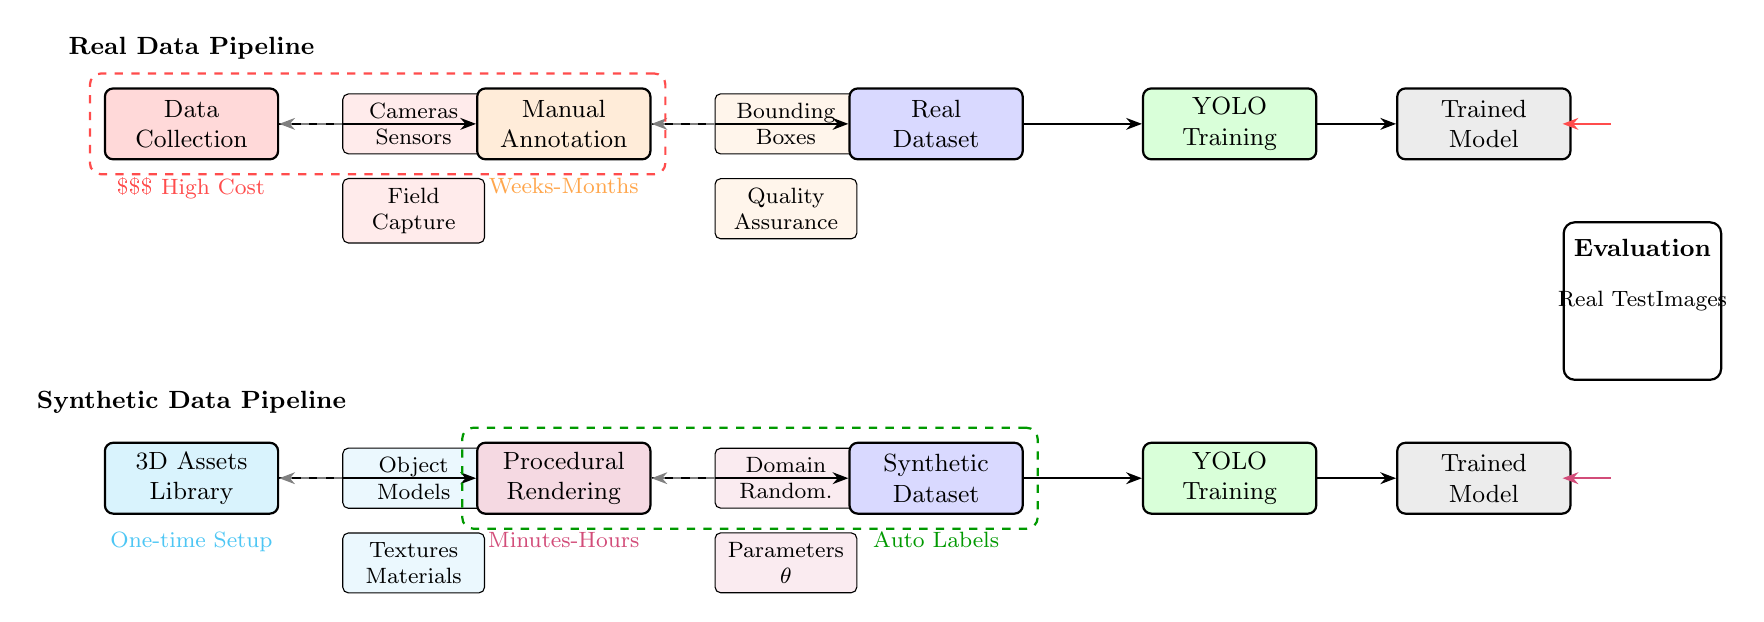
\begin{tikzpicture}[
    node distance=1.2cm and 1.5cm,
    every node/.style={font=\small},
    box/.style={rectangle, draw, thick, minimum width=2.2cm, minimum height=0.9cm, align=center, rounded corners=3pt},
    smallbox/.style={rectangle, draw, minimum width=1.8cm, minimum height=0.7cm, align=center, rounded corners=2pt, font=\footnotesize},
    arrow/.style={-{Stealth[length=2mm]}, thick},
    label/.style={font=\footnotesize},
    title/.style={font=\bfseries\small}
]

% ============ REAL DATA PIPELINE (TOP) ============
\node[title] at (0, 0) {Real Data Pipeline};

% Data collection
\node[box, fill=red!15, below=0.5cm of {(0,0)}] (real_collect) {Data\\Collection};
\node[smallbox, fill=red!8, right=0.8cm of real_collect] (camera) {Cameras\\Sensors};
\node[smallbox, fill=red!8, below=0.3cm of camera] (field) {Field\\Capture};

% Annotation
\node[box, fill=orange!15, right=2.5cm of real_collect] (annotate) {Manual\\Annotation};
\node[smallbox, fill=orange!8, right=0.8cm of annotate] (bbox) {Bounding\\Boxes};
\node[smallbox, fill=orange!8, below=0.3cm of bbox] (qa) {Quality\\Assurance};

% Dataset
\node[box, fill=blue!15, right=2.5cm of annotate] (real_dataset) {Real\\Dataset};

% Training
\node[box, fill=green!15, right=1.5cm of real_dataset] (real_train) {YOLO\\Training};

% Cost/time annotations
\node[label, below=0.1cm of real_collect, text=red!70] {\$\$\$ High Cost};
\node[label, below=0.1cm of annotate, text=orange!70] {Weeks-Months};

% Arrows
\draw[arrow] (real_collect) -- (annotate);
\draw[arrow] (annotate) -- (real_dataset);
\draw[arrow] (real_dataset) -- (real_train);
\draw[arrow, dashed, gray] (camera.west) -- (real_collect.east);
\draw[arrow, dashed, gray] (bbox.west) -- (annotate.east);

% ============ SYNTHETIC DATA PIPELINE (BOTTOM) ============
\node[title] at (0, -4.5) {Synthetic Data Pipeline};

% 3D Assets
\node[box, fill=cyan!15, below=0.5cm of {(0,-4.5)}] (assets) {3D Assets\\Library};
\node[smallbox, fill=cyan!8, right=0.8cm of assets] (models) {Object\\Models};
\node[smallbox, fill=cyan!8, below=0.3cm of models] (textures) {Textures\\Materials};

% Rendering
\node[box, fill=purple!15, right=2.5cm of assets] (render) {Procedural\\Rendering};
\node[smallbox, fill=purple!8, right=0.8cm of render] (dr) {Domain\\Random.};
\node[smallbox, fill=purple!8, below=0.3cm of dr] (params) {Parameters\\$\theta$};

% Dataset with auto-annotation
\node[box, fill=blue!15, right=2.5cm of render] (synth_dataset) {Synthetic\\Dataset};
\node[label, below=0.1cm of synth_dataset, text=green!60!black] {Auto Labels};

% Training
\node[box, fill=green!15, right=1.5cm of synth_dataset] (synth_train) {YOLO\\Training};

% Cost/time annotations
\node[label, below=0.1cm of assets, text=cyan!70] {One-time Setup};
\node[label, below=0.1cm of render, text=purple!70] {Minutes-Hours};

% Arrows
\draw[arrow] (assets) -- (render);
\draw[arrow] (render) -- (synth_dataset);
\draw[arrow] (synth_dataset) -- (synth_train);
\draw[arrow, dashed, gray] (models.west) -- (assets.east);
\draw[arrow, dashed, gray] (dr.west) -- (render.east);

% ============ COMPARISON ANNOTATIONS ============
% Scaling indicator
\node[draw, dashed, thick, green!60!black, rounded corners,
      fit=(render)(synth_dataset), inner sep=5pt,
      label={[font=\footnotesize, green!60!black]below:Unlimited Scaling}] {};

% Bottleneck indicator
\node[draw, dashed, thick, red!70, rounded corners,
      fit=(real_collect)(annotate), inner sep=5pt,
      label={[font=\footnotesize, red!70]above:Scalability Bottleneck}] {};

% Connecting outputs to show comparison
\node[box, fill=gray!15, right=1cm of real_train] (real_model) {Trained\\Model};
\node[box, fill=gray!15, right=1cm of synth_train] (synth_model) {Trained\\Model};

\draw[arrow] (real_train) -- (real_model);
\draw[arrow] (synth_train) -- (synth_model);

% Performance comparison
\node[draw, thick, rounded corners, minimum width=2cm, minimum height=2cm,
      right=1cm of {$(real_model)!0.5!(synth_model)$}] (eval) {};
\node[title, text=black] at (eval.north) [below=0.1cm] {Evaluation};
\node[label, text=black] at (eval.center) {Real Test\\Images};

\draw[arrow, red!70] (real_model.east) -- ++(0.5,0) |- (eval.west |- real_model);
\draw[arrow, purple!70] (synth_model.east) -- ++(0.5,0) |- (eval.west |- synth_model);

\end{tikzpicture}
\end{document}
